%%
%% This is file `sample-xelatex.tex',
%% generated with the docstrip utility.
%%

%% The original source files were:
%%
%% samples.dtx  (with options: `sigconf')
%% 
%% IMPORTANT NOTICE:
%% 
%% For the copyright see the source file.
%% 
%% Any modified versions of this file must be renamed
%% with new filenames distinct from sample-sigconf.tex.
%% 
%% For distribution of the original source see the terms
%% for copying and modification in the file samples.dtx.
%% 
%% This generated file may be distributed as long as the
%% original source files, as listed above, are part of the
%% same distribution. (The sources need not necessarily be
%% in the same archive or directory.)
%%
%% The first command in your LaTeX source must be the \documentclass command.
%\documentclass[sigconf]{acmart}
\documentclass[10pt,conference]{IEEEtran}
%\documentclass[sigconf,review,anonymous]{acmart}

% Copyright 2017 Sergei Tikhomirov, MIT License
% https://github.com/s-tikhomirov/solidity-latex-highlighting/

\usepackage{listings, xcolor}

\definecolor{verylightgray}{rgb}{.97,.97,.97}

\lstdefinelanguage{Solidity}{
	keywords=[1]{anonymous, assembly, assert, balance, break, call, callcode, case, catch, class, constant, continue, constructor, contract, debugger, default, delegatecall, delete, do, else, emit, event, experimental, export, external, false, finally, for, function, gas, if, implements, import, in, indexed, instanceof, interface, internal, is, length, library, log0, log1, log2, log3, log4, memory, modifier, new, payable, pragma, private, protected, public, pure, push, require, return, returns, revert, selfdestruct, send, solidity, storage, struct, suicide, super, switch, then, this, throw, transfer, true, try, typeof, using, value, view, while, with, addmod, ecrecover, keccak256, mulmod, ripemd160, sha256, sha3}, % generic keywords including crypto operations
	keywordstyle=[1]\color{blue}\bfseries,
	keywords=[2]{address, bool, byte, bytes, bytes1, bytes2, bytes3, bytes4, bytes5, bytes6, bytes7, bytes8, bytes9, bytes10, bytes11, bytes12, bytes13, bytes14, bytes15, bytes16, bytes17, bytes18, bytes19, bytes20, bytes21, bytes22, bytes23, bytes24, bytes25, bytes26, bytes27, bytes28, bytes29, bytes30, bytes31, bytes32, enum, int, int8, int16, int24, int32, int40, int48, int56, int64, int72, int80, int88, int96, int104, int112, int120, int128, int136, int144, int152, int160, int168, int176, int184, int192, int200, int208, int216, int224, int232, int240, int248, int256, mapping, string, uint, uint8, uint16, uint24, uint32, uint40, uint48, uint56, uint64, uint72, uint80, uint88, uint96, uint104, uint112, uint120, uint128, uint136, uint144, uint152, uint160, uint168, uint176, uint184, uint192, uint200, uint208, uint216, uint224, uint232, uint240, uint248, uint256, var, void, ether, finney, szabo, wei, days, hours, minutes, seconds, weeks, years},	% types; money and time units
	keywordstyle=[2]\color{teal}\bfseries,
	keywords=[3]{block, blockhash, coinbase, difficulty, gaslimit, number, timestamp, msg, data, gas, sender, sig, value, now, tx, gasprice, origin},	% environment variables
	keywordstyle=[3]\color{violet}\bfseries,
	identifierstyle=\color{black},
	sensitive=false,
	comment=[l]{//},
	morecomment=[s]{/*}{*/},
	commentstyle=\color{gray}\ttfamily,
	stringstyle=\color{red}\ttfamily,
	morestring=[b]',
	morestring=[b]"
}

\lstset{
	language=Solidity,
	backgroundcolor=\color{verylightgray},
	extendedchars=true,
	basicstyle=\footnotesize\ttfamily,
	showstringspaces=false,
	showspaces=false,
	numbers=left,
	numberstyle=\footnotesize,
	numbersep=9pt,
	tabsize=2,
	breaklines=true,
	showtabs=false,
	captionpos=b
}
\usepackage{bera}% optional: just to have a nice mono-spaced font

\colorlet{punct}{red!60!black}
\definecolor{background}{HTML}{EEEEEE}
\definecolor{delim}{RGB}{20,105,176}
\colorlet{numb}{magenta!60!black}

\lstdefinelanguage{json}{
    basicstyle=\normalfont\ttfamily,
    numbers=left,
    numberstyle=\scriptsize,
    stepnumber=1,
    numbersep=8pt,
    showstringspaces=false,
    breaklines=true,
    frame=lines,
    backgroundcolor=\color{background},
    literate=
     *{0}{{{\color{numb}0}}}{1}
      {1}{{{\color{numb}1}}}{1}
      {2}{{{\color{numb}2}}}{1}
      {3}{{{\color{numb}3}}}{1}
      {4}{{{\color{numb}4}}}{1}
      {5}{{{\color{numb}5}}}{1}
      {6}{{{\color{numb}6}}}{1}
      {7}{{{\color{numb}7}}}{1}
      {8}{{{\color{numb}8}}}{1}
      {9}{{{\color{numb}9}}}{1}
      {:}{{{\color{punct}{:}}}}{1}
      {,}{{{\color{punct}{,}}}}{1}
      {\{}{{{\color{delim}{\{}}}}{1}
      {\}}{{{\color{delim}{\}}}}}{1}
      {[}{{{\color{delim}{[}}}}{1}
      {]}{{{\color{delim}{]}}}}{1},
}

\IEEEoverridecommandlockouts
% The preceding line is only needed to identify funding in the first footnote. If that is unneeded, please comment it out.
\usepackage{cite}
\usepackage{amsmath,amssymb,amsfonts}
\usepackage{algorithmic}
\usepackage{graphicx}
\usepackage[numbers]{natbib}
\usepackage{textcomp}
\usepackage{xcolor}
\usepackage{listings}
\usepackage{courier}
\usepackage{url}
\usepackage{hyperref}
\usepackage{relsize,xspace}
\usepackage{fancyhdr}%construct and control page headers and footers

\usepackage{listings}
\usepackage{xcolor}

\definecolor{codegreen}{rgb}{0,0.6,0}
\definecolor{codegray}{rgb}{0.5,0.5,0.5}
\definecolor{codepurple}{rgb}{0.58,0,0.82}
\definecolor{backcolour}{rgb}{0.95,0.95,0.92}

\lstdefinestyle{mystyle}{
    backgroundcolor=\color{backcolour},   
    commentstyle=\color{codegreen},
    keywordstyle=\color{magenta},
    numberstyle=\tiny\color{codegray},
    stringstyle=\color{codepurple},
    basicstyle=\ttfamily\footnotesize,
    breakatwhitespace=false,         
    breaklines=true,                 
    captionpos=b,                    
    keepspaces=true,                 
    numbers=left,                    
    numbersep=5pt,                  
    showspaces=false,                
    showstringspaces=false,
    showtabs=false,                  
    tabsize=2
}

\lstset{style=mystyle}
%% NOTE that a single column version may be required for 
%% submission and peer review. This can be done by changing
%% the \doucmentclass[...]{acmart} in this template to 
%% \documentclass[manuscript,screen]{acmart}
%% 
%% To ensure 100% compatibility, please check the white list of
%% approved LaTeX packages to be used with the Master Article Template at
%% https://www.acm.org/publications/taps/whitelist-of-latex-packages 
%% before creating your document. The white list page provides 
%% information on how to submit additional LaTeX packages for 
%% review and adoption.
%% Fonts used in the template cannot be substituted; margin 
%% adjustments are not allowed.
%%
%%
%% \BibTeX command to typeset BibTeX logo in the docs
\AtBeginDocument{%
  \providecommand\BibTeX{{%
    \normalfont B\kern-0.5em{\scshape i\kern-0.25em b}\kern-0.8em\TeX}}}


\begin{document}

%%
%% The "title" command has an optional parameter,
%% allowing the author to define a "short title" to be used in page headers.
\title{Solidity Smart Contracts: Language constructs for control/currency exchange and guards}


% Double blind Workshop - No author information in this version


%\author{
%\IEEEauthorblockN{Darin Verheijke}
%\IEEEauthorblockA{\textit{Department of Computer Science} \\
%\textit{University of Antwerp}\\
%Antwerp, Belgium \\
%darin.verheijke@student.uantwerpen.be}
%\and
%\IEEEauthorblockN{Henrique Rocha}
%\IEEEauthorblockA{\textit{Department of Computer Science} \\
%\textit{Loyola University Maryland}\\
%Baltimore, USA \\
%henrique.rocha@gmail.com}
%}
\author{
\IEEEauthorblockN{Placeholder 1st Author}
\IEEEauthorblockA{\textit{Department 1} \\
\textit{Affiliation 1}\\
City, Country \\
author1@email.com}
\and
\IEEEauthorblockN{Placeholder 2nd Author}
\IEEEauthorblockA{\textit{Department 2} \\
\textit{Affiliation 2}\\
City,  Country \\
author2@email.com}
}


\maketitle

%%
%% The abstract is a short summary of the work to be presented in the
%% article.
\begin{abstract}
    Ethereum is a blockchain platform which enables the use of smart contracts. Smart contracts will execute a set of instructions without intermediary party when called upon, this process happens automatically. The possibility to make calls to another smart contract within a contract allows for potential exploits to occur. In this paper we will discuss and look at how one of these exploits, called the reentrancy attack, is possible. This attack is most well known for The DAO attack in 2016 where almost 55 million dollar got drained by an attacker who made use of this vulnerability in the smart contract. More specifically we will look at the concept in the Solidity programming language which was made specifically for the Ethereum blockchain. Also an overview of the different advantages and disadvantages of the different functions to exchange Ether, the currency used to execute transactions, will be given, how they work and how the call function might allow for certain exploits. The reentrancy vulnerability is still prevalent in smart contracts nowadays and forms a huge threat to applications and their users due to the huge possible financial losses that can happen. This research also includes an analysis of a verified smart contract database that was collected from Etherscan. This was done to detect potential vulnerabilities by looking for the presence of functions that allow for these attacks. Finally, the results of this analysis are discussed and there will be a brief discussion about prevention measures and methods to avoid a reentrancy attack.
\end{abstract}

\begin{IEEEkeywords}
Blockchain,  Smart Contracts, Solidity,  Reentrancy,  Guards.
\end{IEEEkeywords}


\section{Introduction}
A blockchain is an append-only transactional database where the information is structured together in groups, also known as blocks \cite{smart_inspect, smarter}. Each block has certain storage capacities and is chained onto the previous filled block, thus forming a blockchain. Another way to define it is a shared, immutable ledger that records transactions which can be used to track different assets. Most notable uses of this blockchain technology are the cryptocurrencies Bitcoin\cite{article} and Ether \cite{ethereum, white_paper} on the Ethereum network. One important difference between these two blockchain platforms is that Ethereum enables the deployment of smart contracts. 

A smart contract is a contract which executes automatically when called upon where the terms between the two parties is written in code (on the blockchain). These contracts then run when a function is called and the conditions for that function are met and can be used to automate executions of agreements without any intermediary party \cite{criminal, 10.1145/2993600.2993611, smarter}. In their simplest form a contract is just a collection of functions. Interesting to note is that all smart contract transactions are traceable, transparent and also irreversible \cite{smart_inspect, smarter}.

A common functionality of smart contracts is the possibility to make calls to another contract on the same blockchain platform. This however needs to be done with caution as untrusted contracts can not only introduce errors but also risks as the contract or call may execute malicious code and exploit vulnerabilities. Every call transfers execution control to the called contract.

One of these dangers when calling an external contract is called reentrancy and is one of the most well known attacks due to the DAO Attack on June 2016 where around 3.6 million Ether was taken which equated to around \$50 million dollar at the time \cite{10.1007/978-3-662-54455-6_8}. This exploit is cemented in the history of Ethereum as it resulted into Ethereum being forked into Ethereum Classic and the Ethereum we know today. The original version of this attack involved functions that would be called repeatedly before the first function was finished. 

Solidity is one of the major programming languages for smart contracts on Ethereum. To avoid these exploits there have been introduced some best practices. More specifically the function call() was to be replaced by the more safe functions transfer() and send().  However, recently there has been a switch back to the call() function with the introduction of EIP 1884 \cite{eip1884}.  Other precautions instead must be taken to prevent reentrancy attacks, one recommendation is making use of safe code patterns and using guard constructs. 

In this paper, we will investigate how these calling functions are used in practice and if they are still commonly used for the current smart contracts being deployed in the Ethereum network.  We collected a dataset of 26,800 unique open-source verified smart contracts from Etherscan (from 2012-07-07 to 2022-01-06). 




\section{Background}
An introduction to some important concepts such as blockchain, the consensus mechanism used in Ethereum, smart contracts and reentrancy attacks is given. The scope of these concepts will be kept to the Ethereum blockchain and one of its programming languages Solidity \cite{solidity}.


\subsection{Ethereum \& Smart contracts}
Ethereum differs from Bitcoin in that it enables the deployment of smart contracts and decentralized applications also known as dApps with built-in economic functions. While bitcoin its primary focus is to be a digital currency payment network, Ethereum is designed to be a general-purpose programmable blockchain that runs a virtual machine capable of executing code.
Ether is the currency used to complete transactions on the network and is used as a way to meter and constrain execution resource costs. In comparison to bitcoin, Ether is designed to be a utility currency which is used to call transactions on the Ethereum platform as a sort of fee \cite{mastering}. % Ethereum has two account types, Externally-owned accounts and contracts. Externally-owned accounts can be controlled by anyone who has the private keys to this account while smart contracts are deployed to the network and are controlled by code. 
Smart contracts can be used to create a range of dApps.  An important feature of smart contracts is that when a function is called and the conditions for that function are met there is an automatic execution of the set agreements without any intermediary party \cite{ethereum, white_paper}.

%We take a look at the vending machine example introduced by Nick Szabo, who first coined the term 'Smart contract'\cite{nick}. A simple vending machine will take in coins and via a simple mechanism dispense change and the output we selected. How a vending machine removes the need for a vendor employee, smart contracts remove the intermediary party. Some important properties of smart contracts is that they are immutable and deterministic. Immutable because once deployed due to the nature of how a blockchain works, the code can not change of the smart contract. The only way to modify a smart contract is to deploy a new instance (and thus a new smart contract). Deterministic in the way the outcome after is identical for everyone who, given the same transaction parameters and state of the Ethereum blockchain, executes the contract \cite{white_paper}.


\subsection{Solidity}

Solidity~\cite{solidity} is one of the main languages to code smart contracts in the Ethereum platform.  Solidity is an object-oriented, high-level language which has syntax comparable to C++.  

\subsubsection{Solidity Ether Exchange}

We like to highlight the language constructs use to exchange cryptocurrency among contracts: call, send, and transfer (Table~\ref{tab:freq}).

\begin{table}
\center
  \caption{Solidity Functions to Exchange Ether}
  \label{tab:freq}
  \begin{tabular}{ccl}
    \hline
    Function & Gas Limit & Error Handling\\
    \hline
    call.value & Custom & Returns false on failure\\
    transfer & 2300 & Throws exception on failure\\
    send & 2300 & Returns false on failure\\
  \hline
\end{tabular}
\end{table}

The call function is a low-level interface for sending a message to a contract and it is also a way to send Ether to another address.  The call function transfers the execution control to the called contract and the caller can forward any amount of gas.  Therefore,  the call function has the potential to introduce vulnerabilities, most notably reentrancy.  

The transfer method was first introduced in the version 0.4.10 (May 2017) of the Solidity language.  It provides a safe-by-design method to transfer cryptocurrency.  Even though, this method also transfers the execution control to the caller,  it has a gas limit which prevents abuse.  If the transfers fails,  an exception is raised, which also adds to the security of this method as the exception reverts the transaction.  Due to automatically reverting in case of errors, the transfer function is recommended in most cases. 

The send function can be seem as a lower level implementation of transfer. Similar to transfer,  it provides a safe-by-design function to transfer cryptocurrency,  with a gas limit to prevent exploits. The major difference between send and transfer, is that send returns false if it fails, delegating the error handling to the developer.

\subsubsection{Solidity Guards}

Guards are language constructs to prevent access or revert a transaction.  In Solidity,  different guards have been introduced to the language over different versions such as Require,  and Assert.



\subsection{Reentrancy attack}

The call function has some vulnerabilities.  Every call to another contract transfers execution control to the called contract. Untrusted contracts may introduce and execute malicious code or exploit vulnerabilities.  One of these major vulnerabilities is called the reentrancy attack, which takes advantage of the transfer of execution control by making recursive calls back to the original contract and repeating executions and creating new transactions. 

The two main types of reentrancy attacks are single function and cross-function: Single function,  and Cross-function.

\subsubsection{Single function reentrancy attack}
This version repeatedly calls the involved function before the first invocation of the function is finished.  Listing~\ref{lst:reentrancy1} shows a code snipped with this exploit.

\begin{lstlisting}[language=Solidity, caption=Single function reentrancy attack, label=lst:reentrancy1]
mapping (address => uint) private userBalances;

function withdrawBalance() public {
    uint amountToWithdraw = userBalances[msg.sender];
    (bool succes, ) = msg.sender.call.value(amountToWithdraw)("");
    require(success);
    userBalances[msg.sender] = 0;
    }
// Fallback function which gets executed
function () public payable {
    withdrawBalance()
}
\end{lstlisting}

In this example an attacker can recursively call the \texttt{withdrawBalance()} function and drain the whole contract as the user's balance is only set to 0 at the very end of the function.

\subsubsection{Cross-function reentrancy attack}
When a function shares a state with another function there is a possibility of a cross-function reentrancy attack.  Listing~\ref{lst:reentrancy2}  shows a code snipped with a cross-function reentrancy vulnerability. 
\begin{lstlisting}[language=Solidity, caption=Cross-function reentrancy attack, label=lst:reentrancy2]
mapping (address => uint) private userBalances;

function transfer(address to, uint amount) {
    if (userBalances[msg.sender] >= amount) {
        userBalances[to] += amount;
        userBalances[msg.sender] -= amount;
        }
    }
function withdrawBalance() public {
    uint amountToWithdraw = userBalances[msg.sender];
    (bool succes, ) = msg.sender.call.value(amountToWithdraw)("");
    require(success);
    userBalances[msg.sender] = 0;
}

\end{lstlisting}
Here the attacker will call the transfer function when the code is executed on an external call in \texttt{withdrawBalance()},  again the user's balance is not yet set to 0 and thus they will be able to transfer tokens again. A simple solution to both these types of attacks is updating the balance before transferring control to another function or contract.  Another simple solution would be to use transfer or send (the safer-by-design constructs) instead of call.



\section{Study Design}
\subsection{Dataset}

We collected verified smart contracts from Etherscan\footnote{\url{etherscan.io/contractsVerified}} which is a block explorer and analytic platform for Ethereum. Etherscan verified contracts allows the public to audit and read contracts as it has to be made publicly available to be granted the verified status. Etherscan does not give access to a complete dataset of verified smart contracts but rather has an open source database of the latest 10,000-5,000 smart contracts that were verified. Therefore, we gathered the latest contracts from time to time, over a period of six months (2021-07-07 to 2022-01-06) to build our dataset.

Then, we did the following pre-processing steps in our dataset: (i) remove all duplicated\footnote{We removed contracts with the same address in the Ethereum blockchain. We did not verified whether the contracts with the same name have the same source code. Since these contracts have different addresses, they are considered separate entities in the blockchain platform.} contracts; (ii) remove contracts not written in Solidity; (iii) removed contracts with zero lines of code. After removing those contracts, we had a total of 26,800 unique verified solidity smart contracts. This dataset is publicly available.\footnote{\url{https://bit.ly/3fyOgBD}, the link has been properly anonymized for the reviewers to download the dataset spreadsheet with the name and address of the contracts and not break the double-blind review process.} 

Figure~\ref{fig:dataset} shows the amount of contracts per month in our dataset. The month refers to the date the contract was verified in Etherscan, and not the date it was deployed in the Ethereum network. 

\begin{figure}[h]
  \centering
  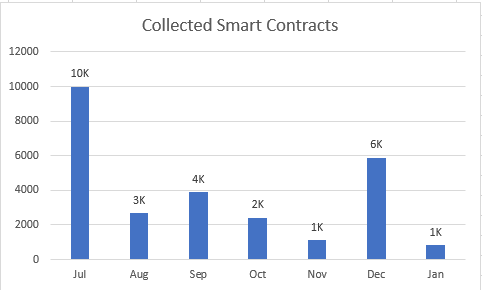
\includegraphics[width=\linewidth]{img/collected_contracts.PNG}
  \caption{Our dataset of verified smart contracts per month after the pre-processing steps. The label on top of each bar is rounded to closest thousand.}
  \label{fig:dataset}
\end{figure}

\subsection{Method}

We use the Etherscan API~\cite{etherscan_api} to retrieve the source codes for each contract in our dataset. Listing~\ref{lst:api} shows an example of the API call used to acquire the contract source code. 
\begin{lstlisting}[language=solidity, caption=Etherscan API call, label={lst:api}]
https://api.etherscan.io/api?module=contract
   &action=getsourcecode
   &address=0xAddress // The contract address
   &apikey=YourApiKeyToken // Your API key
\end{lstlisting}

Then, we analyzed each contract characteristics (lines of code, solidity version) and language constructs looking specifically for Ether exchange functions (call, send, and transfer) and guards (require, and assert). 

\section{Analysis and Results}

\subsection{General Code Characteristics}

First, we show some general characteristics on our dataset.
Table~\ref{tab:loc} shows the general statistics considering the lines of code on the contract. We can see that the contracts in our dataset are small in lines of codes. That is expected, as smart contract code tends to be smaller when compared to software code in other domains. ** Which contract is the biggest? an example of the smallest contract **.

\begin{table}
\center
  \caption{Lines of Code (LoC)}
  \label{tab:loc}
  \begin{tabular}{c c c c c}
    \hline
    Min & Median & Average & Std. Dev. & Max \\
    \hline
   1 & 547 & 739 & 678 & 9,452 \\
  \hline
\end{tabular}
\end{table}

Table~\ref{tab:major-versions} shows the contracts categorized by their major Solidity version. Most contracts are from the latest Solidity version, 0.8.x. The oldest Solidity version to appear in our dataset is 0.4.x which has the fewer amount of contracts.

\begin{table}
\center
  \caption{Solidity Major Versions}
  \label{tab:major-versions}
  \begin{tabular}{crr}
    \hline
    Solidity Version & \# Contracts & Percentage\\
    \hline
    0.8.x & 14,869 &55.48\%\\
    0.6.x & 5,839 &21.79\%\\
    0.5.x & 2,954 &11.02\%\\
    0.7.x & 2,454 &09.16\%\\
    0.4.x & 684 &02.55\%\\
  \hline
\end{tabular}
\end{table}

Figure~\ref{fig:minor-versions} shows the top-10 solidity versions (major and minor) in our contracts. The versions with most contracts are 0.8.4 (18.7\%), 0.6.12 (17.1\%), and 0.8.7 (15.3\%). Together these three versions compose over 50\% of the contracts in our dataset.

\begin{figure}[h]
  \centering
  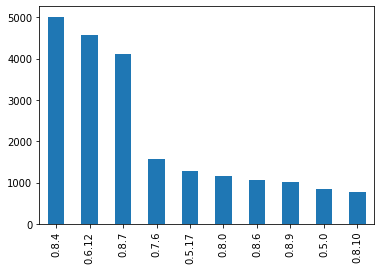
\includegraphics[width=\linewidth]{img/versions_v3.png}
  \caption{Top-10 Solidity versions in the database.}
  %\description{Solidity Compiler Version}
  \label{fig:minor-versions}
\end{figure}


We will now dive deeper into the source contracts themselves and have a look at the different functionality, more specifically we will count the amount of times we find a call, send, and transfer function which as mentioned earlier are the main methods to exchange Ether in a Solidity smart contract. We will also calculate the amount of times a require, assert and throw function has been called in order to see how many of this contracts make use of guards. Table \ref{tab:stats} shows us the different statistics for the collected database. We notice that almost all contracts have some form of a guard pattern with a require function. Only 270 contracts actually have a call.value function which shows us that they may have a potential reentrancy attack. 

\begin{table}
  \caption{Statistics}
  \label{tab:stats}
  \begin{tabular}{ccl}
    \hline
    Function & \# Contracts & \# Functions\\
    \hline
    Call&270&384\\
    Send&9176&17,814\\
    Transfer&647&1059\\
    Require&26,191&622,701\\
    Assert&7279&10,507\\
    Throws&4174&10,590\\
    \hline
\end{tabular}
\end{table}

\subsection{Ether Exchange Functions}

The next experiment will focus more on those contracts that contain a call.value function, all previous statistics will be recalculated for only the smart contracts containing a call.value function to see if there are any similarities but first we will take a look at which version is used most in these contracts.
Figure \ref{fig:call_version}. The most used version is v0.5.17 which was the 5th most used version in all our contracts. A more interesting finding is that there are only 4 contracts above v0.6 that contain a call function of which 3 are from the compiler version that was most used by the complete database namely v0.8.4. For the line of code statistics we get the following values:
\begin{itemize}
    \item Average: 1050
    \item Median: 761
    \item Standard deviation: 1079
    \item Min: 31
    \item Max: 6535
\end{itemize}
We notice that these smart contracts on average are of a relatively bigger size in comparison with a regular contract.
Table \ref{tab:call} will now show us different statistics for this specific selection of contracts that only contain a call.value function. In this sub selection of contracts a call function is called about 1.4 times on average in a contract and a total of 384 call functions were called in 270 contracts with the highest amount of calls in a single contract being 14. An interesting thing to note is that the average amount of guards is higher for these contracts, this shows us that a guard pattern has been potentially used in cases where a call.value function has been used and are signs that most of these contracts are probably correctly implemented. 

\begin{figure}[h]
  \centering
  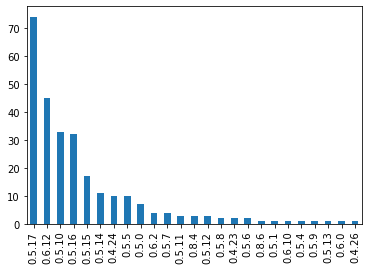
\includegraphics[width=\linewidth]{img/versions_call_v3_total.png}
  \caption{An overview of all the specific compiler versions used in contracts that contain a call.value function. }
  %\description{Solidity Compiler Version}
  \label{fig:call_version}
\end{figure}

\begin{table}
  \caption{Statistics of Contracts containing call function}
  \label{tab:call}
  \begin{tabular}{ccl}
    \hline
    Function & \# Contracts & \# Functions\\
    \hline
    Send&153&495\\
    Transfer&18&51\\
    Require&270&11932\\
    Assert&192&333\\
    Throws&163&324\\
    \hline
    Function & Avg/contract\\
    \hline
    Send&1.83\\
    Transfer&0.19\\
    Require&44.19\\
    Assert&1.23\\
    Throws&1.2\\
  \hline
\end{tabular}
\end{table}

We will do a similar analysis on both the send and transfer function. Looking at the versions in Figure \ref{fig:send_version} we can see that for the send function the top 5 versions are completely similar to the top 5 versions of the whole contract database. This is partly due to the fact that 66\% of the contracts of our whole database have a send function. If we look at the versions of transfer in Figure \ref{fig:transfer_version} we notice that both v0.8.4 and 0.6.12 are not even in the top 10 versions which is interesting. A version that also showed up in the top 10 of call versions namely v0.4.24 shows up here. This signifies that both call and transfer functions were used more often in v0.4 and that since then there was a shift to the send function. 

\begin{figure}[h]
  \centering
  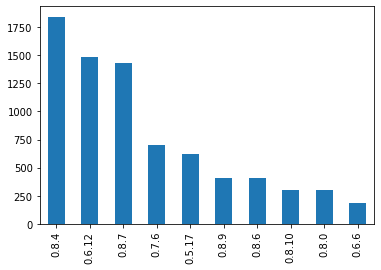
\includegraphics[width=\linewidth]{img/sends_versions.png}
  \caption{An overview of all the specific compiler versions used in contracts that contain a send function. }
  %\description{Solidity Compiler Version (Sends)}
  \label{fig:send_version}
\end{figure}

\begin{figure}[h]
  \centering
  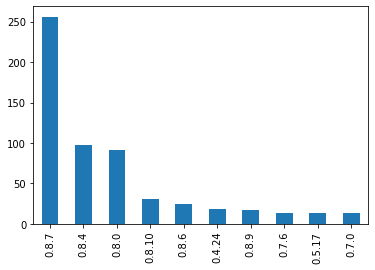
\includegraphics[width=\linewidth]{img/transfers_versions.png}
  \caption{An overview of all the specific compiler versions used in contracts that contain a transfer function. }
  %\description{Solidity Compiler Version (Transfers)}
  \label{fig:transfer_version}
\end{figure}

If we calculate the LOC statistics for both contracts containing send functions and contracts containing transfer functions we get the statistics in Table \ref{tab:loc}. Contracts containing a transfer function seem to be a lot longer on average (almost twice as long) in comparison with the average length of a smart contract. A contract containing a send function is pretty similar in length in comparison with the average smart contract.
\begin{table}
  \caption{LOC Statistics for send and transfer}
  \label{tab:loc}
  \begin{tabular}{ccl}
    \hline
    Statistic & Send & Transfer\\
    \hline
    Average&832&1453\\
    Mean&553&1378\\
    Std Dev&741.78&841.18\\
    Min&10&20\\
    Max&9452&9452\\
  \hline
\end{tabular}
\end{table}

Of all contracts containing a send functions there are almost on average two send functions per contract with the highest amount of send functions used in any contract being 68. This is by far the most used way of transferring Ether in the database that we collected. The transfer function is present in a lot less contracts but when it is used, the average of times it is in a contract is around 1.63 times with the highest amount being 12. 
We will now look at the different functions present in both cases in a similar way we did for the call function for which the results can be found in Table \ref{tab:send} and Table \ref{tab:transfer}. For the contracts containing a send function we notice that they almost always include atleast one require guard as well. The average of require guards used in a contract containing a transfer function is however higher in comparison with the average of contracts that contain a send function. We can also see that the average of both assert guards and throws are higher for contracts containing a send function than the transfer function. If we now compare some of these statistics to the numbers of the contracts containing a call function we immediately see that those contracts have a lot more guards. These due to the fact that both transfer and send are considered safer functions and thus a call function by design will need to utilize more guards for it to not be exploited.

\begin{table}
  \caption{Statistics of Contracts containing send function}
  \label{tab:send}
  \begin{tabular}{ccl}
    \hline
    Function & \# Contracts & \# Functions\\
    \hline
    Call&153&226\\
    Transfer&107&251\\
    Require&9060&256835\\
    Assert&2722&4789\\
    Throws&1507&4338\\
    \hline
    Function & Avg/contract\\
    \hline
    Call&0.0246\\
    Transfer&0.0274\\
    Require&27.9898\\
    Assert&0.5219\\
    Throws&0.4727\\
  \hline
\end{tabular}
\end{table}

\begin{table}
  \caption{Statistics of Contracts containing transfer function}
  \label{tab:transfer}
  \begin{tabular}{ccl}
    \hline
    Function & \# Contracts & \# Functions\\
    \hline
    Call&18&20\\
    Send&107&234\\
    Require&647&25058\\
    Assert&63&166\\
    Throws&53&224\\
    \hline
    Function & Avg/contract\\
    \hline
    Call&0.0309\\
    Send&0.3616\\
    Require&38.7295\\
    Assert&0.2566\\
    Throws&0.3462\\
  \hline
\end{tabular}
\end{table}
\section{Related work}


Juels, Kosba and Shi\cite{criminal} investigate the risk of smart contracts fueling new criminal ecosystems . They show how a Criminal Smart Contract can facilitate leakage of confidential information, theft of cryptographic keys and more, showing the urgency of creating safeguards against these CSCs. They look at questions like how practical these new crimes will be, whether these CSCs enable a wider range of new crimes in comparison to earlier cryptocurrencies such as Bitcoin and what advantages they offer to criminals in comparison with the conventional online systems. 


Luu et al.  \cite{smarter} also investigate and introduce several security problems to manipulate smart contracts in an attempt to gain profit and propose ways to enhance the operational semantics of Ethereum. A focus is put on the semantic gap between the assumption contract writers make about the underlying execution semantics and the actual semantics of the contract are made as a reason for these security flaws. A tool OYENTE is also provided to detect bugs which is a symbolic execution tool. The model works directly with Ethereum virtual machine byte code and thus does not have a need for a higher level representation such as Solidity. An evaluation of OYENTE on 19366 smart contracts is given where 8333 contracts were documented as potentially having bugs.

Mense and Flatscher \cite{security} summarize known vulnerabilities found by literature research and analysis such as external calls, gasless sends, mishandled exceptions and reentrancy. They also compare code analysis tools for their ability to identify vulnerabilities in smart contracts based on a taxonomy for vulnerabilities. The results of their paper show that reentrancy ranks the highest among the vulnerabilities that they have discussed and is detected by most of the tools used. They then delve deeper into the DAO hack aswell. 


Liu et al. \cite{reguard} present ReGuard which is a fuzzing-based analyzer to automatically detect reentrancy bugs in Ethereum smart contracts. They iteratively generate random (but diverse) transactions, this is called fuzz testing. Then based on the runtime they will identify reentrancy vulnerabilities in a contract. How the architecture works is they parse a smart contracts source or binary code to an intermediate representation which will then be transformed to C++, keeping the original behavior. Together with a runtime library, ReGuard executes the contract and runs an analysis of the operations for any reentrancy attacks.


SmartCheck is an extensible static analysis tool to detect code issues in Solidity by Tikhomirov et al.\cite{smartcheck} where they translate Solidity into an XML-based representation and check it against XPath patterns. They also used a real world dataset to evaluate their tool and also make a comparison to the earlier mentioned Oyente. 


Samreen and Alalfi  \cite{survey} explain eight vulnerabilities by looking at past exploitation case scenarios and review some of the available tools and applications to detect these vulnerabilities. For each case they discuss the vulnerability exploited, the tactic used as well as the financial loss what happened. A coverage is given of some preventive techniques as protection against some of these exploits. The tools/frameworks they discuss adopt either a form of static analysis such as symbolic execution and control flow graph construction or dynamic analysis such as the fuzzing testing or tracing the sequence of instructions that are executed at run time. 

Tantikul and Ngamsuriyaroj \cite{icissp20} investigate a more recent state of the vulnerabilities of smart contracts. Their research consists of going through a database of verified smart contracts and checking common occurrences as well as trends of vulnerabilities. An analysis is done using both Oyente and Smartcheck and common characteristics of vulnerable smart contracts are identified. A correlation computation is done via Pearson's correlation in order to detect how often any pair of vulnerabilities will be found on the same smart contract. Their results show that overflow and underflow have the highest correlation. Another relation found is the timestamp dependency and transaction ordering which might be caused by malicious miners.  

Bragagnolo, Rocha, Denker and Ducasse \cite{rocha} address the lack of inspectability of a deployed smart contact. They do this by analyzing the state of the contract using different decompilation techniques. Their solution SmartInspect is an inspector based on pluggable property reflection. Their approach of utilizing mirrors generated from an analysis of Solidity source code allows access to unstructured information from a deployed smart contract in a structured way. This can be done without a need to redeploy or develop additional code for decoding. 

Wang et al. \cite{contractward} evaluate a set of real-world smart contracts with ContractWard which uses machine learning techniques to detect vulnerabilities in smart contracts. Their idea was proposed due to existing detection methods being mainly based on symbolic execution or analysis which are very time-consuming. The system extracts dimensional bigram features from simplified operation codes to construct a feature space and is able to get a predictive recall and precision of over 96\% based on their dataset of 49502 smart contracts on 6 vulnerabilities.

A deep-learning based approach is used by Qian et al. \cite{automated}. The aim is to precisely detect reentrancy bugs using a bidirectional long-short term memory with attention mechanism. They also propose using a contract snippet as another way to represent a smart contract only capturing key semantic sentences which contain related and critical information such as control flow and data dependencies. These are then used as input to the sequential models. They show that this deep-learning approach outperforms other state-of-the-art smart contract vulnerability tools.

Slither by Feist et al. \cite{slither} is a static analysis framework that converts Solidity smart contracts into an intermediate representation which they call SlithIR. Static Single Assignment forms are used aswell as a reduced instruction set for ease of implementation. Their framework has use cases in automated detection of vulnerabilities, detection of code optimization opportunities, improvement of clarity and ease of understanding of the contracts. An evaluation of the proposed frameworks capabilities is done using a set of real-world smart contracts. 

%%
%% The next two lines define the bibliography style to be used, and
%% the bibliography file.

\bibliographystyle{IEEEtranN}
\bibliography{references}

%\endinput
\end{document}

